% !TeX root = ../main.tex

Nel capitolo \ref{ch:ch2} sono stati individuati gli step che compongono il processo di sviluppo. Per poter adottare e automatizzare questo processo sono necessari molti strumenti che riguardano sia la parte di sviluppo (\textit{Dev}), come ad esempio strumenti di versionamento, ambienti di sviluppo e SDK, che la parte operativa (\textit{Ops}), come ad esempio strumenti di build automation e package registry. In questo capitolo viene descritta l'infrastruttura aziendale a supporto del processo di sviluppo e i principali tools adottati come vincolo tecnologico per il progetto di tesi.

\section{Infrastruttura}
L'infrastruttura aziendale a supporto di tutti i processi di sviluppo è di tipo multi-cloud ibrido. E' composta infatti da servizi completamente gestiti da diversi cloud provider, da servizi ospitati sul cloud ma auto-gestiti e da installazioni interne su hardware proprietario. I seguenti rappresentano tutti i componenti infrastrutturali necessari al processo di sviluppo progettato per applicazioni mobile e descritto successivamente nel capitolo \ref{ch:ch4}:
\begin{itemize}
    \item \textit{SonarQube, Nexus Sonatype, GitLab Runner (Linux)} - Servizi disponibili per tutti i team di sviluppo Maggioli e ospitati su Google Cloud.
    \item \textit{GitLab Cloud} - Licenza aziendale per tutti gli sviluppatori Maggioli.
    \item \textit{Cluster Kubernetes, Container Registry} - Servizi disponibili per il solo team di Ricerca e Sviluppo e ospitati su Microsoft Azure.
    \item \textit{Google Play Console, Testflight} - Servizi specifici per lo sviluppo di applicazioni Android e iOS, per i quali sono stati sottoscritti account developer appositi per questo progetto di tesi.
    \item \textit{GitLab Runner (MacOS)} - Servizio interno per l'esecuzione delle pipeline in ambiente Apple, specifico per questo progetto di tesi.
\end{itemize}

\begin{figure}[H]
\centering
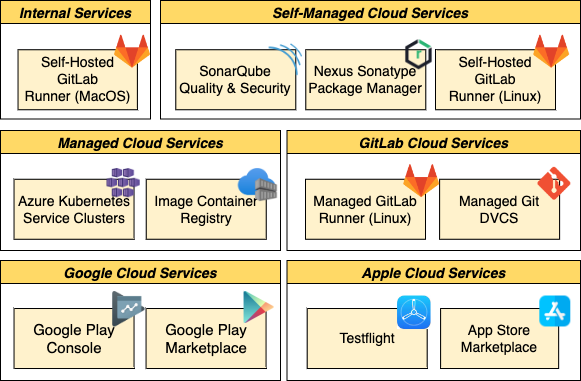
\includegraphics[width=0.8\textwidth]{img/tesi-3-infra.drawio.png}
\caption{Componenti della infrastruttura necessaria a supporto del processo di sviluppo progettato}
\end{figure}

\section{MacOS GitLab Runner (Self-Hosted)}
Ogni job di ogni stage definito in una pipeline viene eseguito da un componente software chiamato \textit{runner}. Tramite il modello client-server il runner interroga continuamente il server (ovvero GitLab) per ottenere le informazioni necessarie all'esecuzione dei job. La politica di scheduling dei job fra i vari runner è definita lato server ma può essere pilotata tramite il concetto di \textit{tag}.

\begin{figure}[H]
\centering
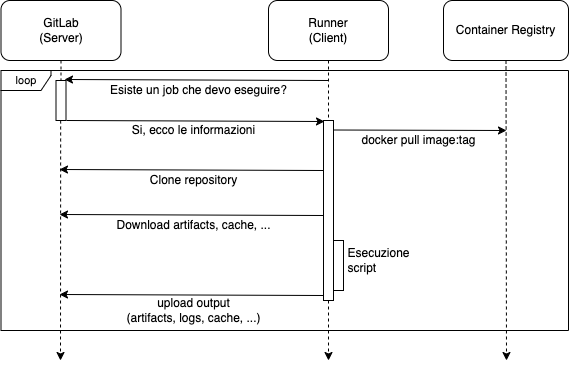
\includegraphics[width=0.8\textwidth]{img/tesi-17-runner.drawio.png}
\caption{Diagramma di sequenza GitLab Runner (Docker Executor)}
\label{fig:archrunner}
\end{figure}

In base a chi lo gestisce, il runner può essere:
\begin{itemize}
    \item \textit{Managed} - Runner gestito da GitLab e fornito in modalità as-a-Service. E' soggetto ad alcune restrizioni di utilizzo che dipendono dal piano di licenza sottoscritto: tipicamente questi limiti coinvolgono il tempo di esecuzione e lo spazio di archiviazione. Come vantaggio non richiedono alcuno sforzo nella loro configurazione e gestione
    \item \textit{Self-Hosted} - Runner gestito interamente dall'utente (installazione, configurazione, registrazione, manutenzione, aggiornamento, ...). A differenza dei runner managed con questa modalità le fasi di configurazione e gestione sono più complesse ma non ci sono vincoli sull'utilizzo in termini di risorse (CPU e storage).
\end{itemize}

La toolchain per lo sviluppo di applicazioni iOS è interamente di proprietà Apple e richiede l'utilizzo di macchine MacOS, definendo una serie di vincoli per quanto riguarda sia lo sviluppo che l'automazione del processo. Per limitare i costi e aumentare la conoscenza del team di ricerca e sviluppo anche in ambito applicazioni mobile è stato adottato il runner self-hosted.

\subsection{Shell Executor}
L'esecuzione dei job avviene in modo asincrono tramite l'esecuzione di task sottoposti ad un executor. Una entità master si occupa quindi di ottenere i job da far eseguire all'executor, il quale restituisce il risultato una volta terminato. Il grado di concorrenza dell'executor, ovvero il numero di job che possono essere eseguiti in parallelo, è configurabile dalle impostazioni del runner. Le principali tipologie di executor sono\footnote{\url{https://docs.gitlab.com/runner/executors/}}:
\begin{itemize}
    \item \textit{Shell} - Per ogni job viene aperta una shell sulla macchina host in cui è in esecuzione il runner. Tutte le dipendenze necessarie alla esecuzione dei job devono essere installate sulla macchina.
    \item \textit{Container} - L'ambiente di esecuzione dei job è circoscritto all'interno di un container, sia nel caso dell'executor Docker che dell'executor Kubernetes (Pods). Tutte le dipendenze necessarie alla esecuzione dei job devono essere installate all'interno del container utilizzato.
    \item \textit{Virtual Machine} - I job vengono eseguiti all'interno di virtual machine, VirtualBox o Parallels, già preconfigurate.
\end{itemize}

Data la assenza di container basati su sistema operativo MacOS, l'unica opzione accettabile è quella dell'executor di tipo shell attraverso l'installazione\footnote{\url{https://docs.gitlab.com/runner/install/osx.html}} di un runner su una macchina fisica Apple all'interno della rete privata aziendale Maggioli.

\subsection{Configurazione}
A prescindere dalla tipologia di executor, per l'utilizzo di un runner GitLab self-hosted è necessario effettuarne installazione, configurazione e avvio. Nel caso di un executor shell è necessario installare il binario\footnote{\url{https://gitlab-runner-downloads.s3.amazonaws.com/latest/binaries/gitlab-runner-darwin-arm64}} mentre nel caso di un executor Docker/Kubernetes è necessario effettuare il deploy del container\footnote{\url{https://hub.docker.com/r/gitlab/gitlab-runner}}. La fase di configurazione del runner varia a seconda del tipo di executor. Per la tipologia di runner scelta per questo progetto di tesi gli aspetti principali configurati sono:
\begin{itemize}
    \item \textit{Registrazione} - Come descritto nella architettura (figura \ref{fig:archrunner}) un runner GitLab interroga continuamente il server per ottenere job da eseguire. E' necessario specificare sia l'indirizzo URL del server GitLab che il gruppo o il progetto per il quale il runner deve eseguire i job. Altri parametri come \textit{locked}, \textit{tag-list} e \textit{run-untagged} sono stati utilizzati per limitare l'accesso del runner al solo repository utilizzato per questo progetto di tesi.
    \begin{listing}[H]
    \inputminted{bash}{code/4-macos-runner-setup}
    \caption{Comandi bash utilizzati per l'installazione e la configurazione di un runner MacOS}
    \end{listing}
    \item \textit{Cache Condivisa} - Permette di condividere uno storage cloud (Google Cloud Storage Buckets in questo caso) per il caching di tutte le dipendenze comuni tra i vari job eseguiti concorrentemente dal runner. L'utilizzo di cache condivisa con un executor shell comporta un vantaggio nell'utilizzo dello spazio disco della macchina in cui è in esecuzione il runner ma non nel tempo di esecuzione delle pipeline, il quale sarebbe molto più ridotto nel caso di cache locale.
\end{itemize}

\begin{listing}[H]
\inputminted{toml}{code/4-macos-runner-config}
\caption{File di configurazione (\textit{config.toml}) generato al momento della registrazione del runner}
\end{listing}

\subsection{Pipeline As Code}
% descrivere cos'è e i vantaggi
% metodo per definire la pipeline (cos'è una pipeline) e sottomettere i job al runner

\section{Kotlin Multiplatform Mobile}
Kotlin Multiplatform Mobile\footnote{\url{https://kotlinlang.org/lp/mobile/}} (KMM) è un framework per lo sviluppo di app iOS e Android basato sul concetto di condivisione della logica applicativa mantenendo lo sviluppo nativo della UX/UI\footnote{User Experience/User Interface}. Consiste in un caso d'uso specifico (e il più diffuso) del framework Kotlin MultiPlatform (KMP), il quale permette di sviluppare il codice in modo agnostico rispetto le piattaforme target e di condividerlo tra differenti piattaforme facendo uso dei tre principali compilatori inclusi nell'ecosistema Kotlin\cite{nagy2022simplifying}:
\begin{itemize}
    \item Kotlin/JVM (Android, Spring, ...)
    \item Kotlin/Native (iOS, macOS, ...)
    \item Kotlin/JS (Web)
\end{itemize}
KMM dipende fortemente dai compilatori Kotlin/JVM (Android) e Kotlin/Native (iOS) e fornisce benefici derivanti sia dallo sviluppo cross-platform che dallo sviluppo nativo:
\begin{itemize}
    \item risparmio di tempo e risorse derivanti dalla condivisione del codice (cross-platform),
    \item alte performance (nativo),
    \item accesso diretto alle funzionalità dei dispositivi hardware senza overhead (nativo).
\end{itemize}

\begin{figure}[H]
\centering
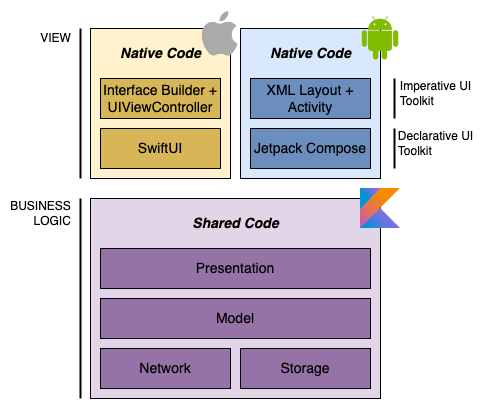
\includegraphics[width=0.7\textwidth]{img/tesi-8-kmm.drawio.png}
\caption{Architettura Kotlin Multiplatform Mobile}
\label{stackKMM}
\end{figure}

Con il rilascio di Kotlin 1.4 (Agosto 2020), KMM è passato dalla fase "\textit{Experimental}" alla fase "\textit{Alpha}" la quale è considerata come fase "\textit{pre-stable}"\footnote{\url{https://kotlinlang.org/docs/components-stability.html\#current-stability-of-kotlin-components}} ma è comunque già stato adottato in produzione per lo sviluppo delle proprie applicazioni mobile da tantissime aziende tra le quali è possibile trovare nomi rilevanti come Netflix, VMware e Philips\footnote{\url{https://kotlinlang.org/lp/mobile/case-studies/}}.\\
In base al risultato dell'indagine di mercato svolta nei primi due quadrimestri del 2021\cite{kmm2}, le porzioni di codice condiviso nelle applicazioni sviluppate con KMM sono:
\begin{itemize}
    \item 85\% Networking
    \item 75\% Data Storage
    \item 70\% Utility (Logging, Analytics, ...)
    \item $\sim$60\% Algoritmi/Computazione
    \item $\sim$55\% State Management
    \item $\sim$50\% Presenters/Controllers/ViewModel
\end{itemize}

\subsection{Kotlin/JVM}
Il compilatore Kotlin/JVM è uno dei due compilatori su cui è basato KMM, utilizzato per la piattaforma Android. Permette di compilare codice Kotlin in bytecode Java (\textit{.class}), il quale può essere eseguito direttamente sulla JVM. Nel caso di Android è necessario un ulteriore passaggio per tradurre il bytecode Java in bytecode Dalvik (\textit{.dex}).

\begin{figure}[H]
\centering
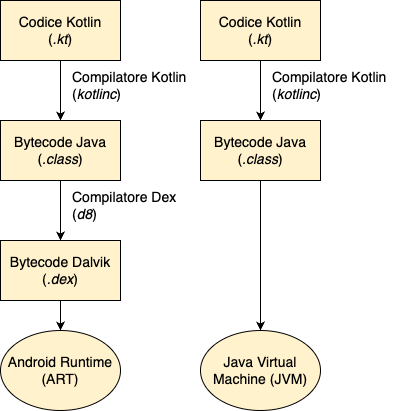
\includegraphics[width=0.55\textwidth]{img/tesi-9-kotlinjvm.drawio.png}
\caption{Fasi di compilazione Kotlin/JVM con piattaforma target Android e JVM}
\end{figure}

\subsection{Kotlin/Native}
Kotlin/Native è il secondo compilatore su cui è basato KMM e viene utilizzato per la piattaforma iOS. A differenza del compilatore Kotlin/JVM, il compilatore Kotlin/Native è progettato per quelle situazioni dove non è possibile o non si vuole avere una VM come nel caso dei dispositivi embedded e della piattaforma iOS. Per fare ciò include un backend basato su \textit{Low Level Virtual Machine} (LLVM)\footnote{\url{https://llvm.org/}}, ovvero il codice Kotlin viene compilato in binari nativi che possono essere eseguiti senza VM\cite{nagy2022simplifying}. Le piattaforme supportate da Kotlin/Native attualmente sono macOS, iOS, tvOS, watchOS, Linux, Windows (MinGW) e Android NDK\footnote{\url{https://kotlinlang.org/docs/native-overview.html\#target-platforms}} e per ognuna di esse esistono differenti architetture. Nel caso di iOS le differenti architetture supportate da KMM sono \textit{Arm64}, \textit{Arm32} e \textit{x64}.
\begin{figure}[H]
\centering
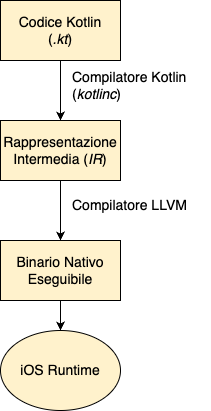
\includegraphics[width=0.45\textwidth]{img/tesi-10-kotlinnative.drawio.png}
\caption{Fasi di compilazione Kotlin/Native con piattaforma target iOS}
\end{figure}
Anche in questo caso sono necessarie due fasi di compilazione: ($i$) il codice Kotlin viene compilato nella \textit{Rappresentazione Intermedia} (IR) LLVM e ($ii$) successivamente compilato nel binario nativo.

\subsection{Expect/Actual}
Quando si sviluppa codice condiviso è spesso necessario definire come determinate funzionalità debbano essere implementate sulla specifica piattaforma target per utilizzare i relativi SDK. Il framework KMP fornisce il meccanismo \textit{expect/actual} per assolvere a questo compito in modo analogo al design pattern \textit{Template Method}:
\begin{itemize}
    \item \textit{Expect} - Astrazione della funzionalità necessaria. Tramite la keywork \textit{expect} si definisce lo scheletro astraendo dalla specifica implementazione.
    \item \textit{Actual} - Implementazione specifica per una determinata piattaforma. Tramite la keywork \textit{actual} si definisce l'implementazione, reificando l'astrazione definita tramite il concetto di \textit{expect}.
\end{itemize}

\begin{listing}[H]
\inputminted{kotlin}{code/3-expectactual}
\caption{Esempio di applicazione expect/actual per ottenere informazioni sulla piattaforma}
\end{listing}

\subsection{Plugin Gradle KMP}
Il plugin Gradle KMP è uno strumento utile per realizzare progetti multiplatform. Fornisce uno specifico DSL\footnote{Domain Specific Language} per definire e configurare i task necessari a compilare il codice condiviso per le relative piattaforme target\footnote{\url{https://kotlinlang.org/docs/multiplatform-dsl-reference.html}}. Al momento la versione latest (stable) del plugin è la \textit{1.6.21}, rilasciata il 19/04/2022\footnote{\url{https://plugins.gradle.org/plugin/org.jetbrains.kotlin.multiplatform/1.6.21}} ma è presente una versione candidata per il rilascio con tag \textit{1.7.0-RC2}.

\begin{listing}[H]
\inputminted{kotlin}{code/3-gradlekmm1}
\caption{Struttura iniziale del file \textit{settings.gradle.kts} nella root di progetto (Kotlin)}
\end{listing}

\begin{listing}[H]
\inputminted{kotlin}{code/3-gradlekmm2}
\caption{Definizione utilizzo Plugin Gradle KMP nel file \textit{build.gradle.kts} del modulo condiviso (Kotlin)}
\end{listing}

\subsubsection{Plugin Tasks}
Il plugin gradle KMM e le relative dipendenze rendono disponibile una vasta serie di task per eseguire differenti elaborazioni sia sul codice della specifica piattaforma target che sul codice condiviso. Alcune delle principali tipologie di task sono:
\begin{itemize}
    \item Build - tasks per build, compile, link
    \item CocoaPods - tasks per la gestione delle dipendenze Swift/Objective-C
    \item Interop - tasks relativi all'utilizzo del \textit{commonizer}\footnote{\url{https://github.com/JetBrains/kotlin/tree/master/native/commonizer}}
    \item Verification tasks - tasks per l'esecuzione dei test
\end{itemize}

\subsubsection{KMM Android Studio IDE Plugin}
L'IDE\footnote{Integrated Development Environment} Android Studio è costruito su IntelliJ, il quale è uno tra gli IDE più diffusi ed è sviluppato da JetBrains. Tramite il plugin KMM, installabile direttamente dal marketplace integrato in Android Studio o dal sito ufficiale JetBrains\footnote{\url{https://plugins.jetbrains.com/plugin/14936-kotlin-multiplatform-mobile/versions/stable}}, si abilita un insieme di funzionalità a supporto dello sviluppo di codice multiplatform, in particolare:
\begin{itemize}
    \item creazione della struttura e della configurazione base per una nuova applicazione multiplatform,
    \item creazione della struttura e della configurazione base per una nuova libreria multiplatform,
    \item integrazione di moduli multiplatform in applicazioni già esistenti.
\end{itemize}

\subsection{Struttura Applicazione KMM}
Una applicazione sviluppata con KMM segue lo stack definito dalla condivisione della business logic e la separazione della UX/UI (figura \ref{stackKMM}). Il modulo \textit{shared} contiene tutta la business logic condivisa, la quale può essere sviluppata tramite l'utilizzo di librerie con supporto nativo al framework KMM, cioè librerie che forniscono già al loro interno specifiche implementazioni per le diverse piattaforme target, oppure tramite l'utilizzo del meccanismo expect/actual come descritto sopra.\\
Nel caso di utilizzo del meccanismo expect/actual è necessario definire le funzionalità nel modulo \textit{commonMain} e fornire le implementazioni per le specifiche piattaforme nei relativi moduli \textit{androidMain} e \textit{iosMain}. Gli stessi concetti vengono applicati per la struttura dei moduli di test: \textit{commonTest}, \textit{androidTest} e \textit{iosTest}.\\
I moduli UX/UI delle relative piattaforme includono il codice condiviso come dipendenza di progetto, in particolare come dipendenza Gradle (\textit{aar}\footnote{Android Archive}) per Android e come dipendenza CocoaPods (Pod) per iOS.

\begin{figure}[H]
\centering
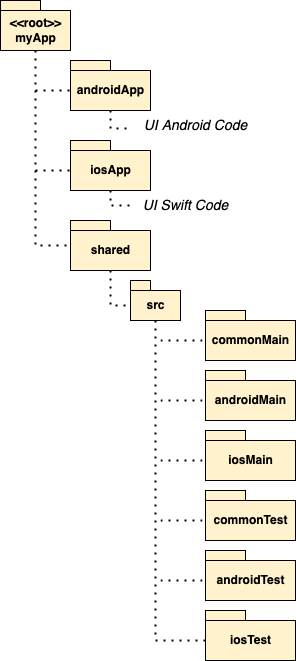
\includegraphics[width=0.4\textwidth]{img/tesi-2-Page-14.drawio.png}
\caption{Fasi di compilazione Kotlin/Native con piattaforma target iOS}
\end{figure}

\section{Fastlane}
Uno fra i tool open source più diffusi a supporto della automazione dello sviluppo di applicazioni mobile, sia Android che iOS, è Fastlane\footnote{\url{https://github.com/fastlane/fastlane}}. L'impiego principale di questo tool sviluppato in Ruby consiste nella automazione della fase di rilascio della applicazione, sia in beta che in produzione, grazie alla gestione di tutti quei task necessari ma dispendiosi in termini di tempo come ad esempio la generazione degli screenshot e la firma digitale del codice (\textit{Code Signing}).\\
Si fa uso dei seguenti concetti per controllare il comportamento di fastlane negli appositi file di configurazione \textit{Fastfile} e \textit{Appfile}:
\begin{itemize}
    \item \textit{Action} - Elaborazioni pre-definite e configurabili tramite passaggio di parametri.
    \item \textit{Lane} - Insieme di action definito dall'utente per descrivere elaborazioni complesse.
\end{itemize}

\begin{listing}[H]
\inputminted{ruby}{code/4-fastlane}
\caption{Esempio di definizione di un lane per il rilascio in versione beta di applicazioni iOS}
\end{listing}

I file \textit{Fastfile} e \textit{Appfile}, i quali risiedono nella cartella \textit{fastlane} nella root di progetto, sono utilizzati rispettivamente per definire configurazioni globali a livello di applicazione e per definire il comportamento di fastlane. Per questo motivo è necessario configurare fastlane per ogni modulo che si intende utilizzare, sia che esso sia una libreria o una applicazione. Nel caso di applicazioni multiplatform è quindi necessario per tutti i tre moduli \textit{shared}, \textit{androidApp} e \textit{iosApp}.\\
Nelle successive descrizioni delle fasi che compongono la pipeline progettata viene indicato come è stato configurato e adottato Fastlane ove utilizzato.